\documentclass{clv2025}

\jvol{vv}
\jnum{nn}
\jyear{2026}
\jinfo{}
\renewcommand{\footmark}{}
\dochead{Position Paper}

\usepackage[T1]{fontenc}
\usepackage[american]{babel}
\usepackage{natbib}
\bibliographystyle{compling}
\usepackage{mathtools}
\usepackage{amssymb}
\usepackage{booktabs}
\usepackage{tabularx}
\usepackage{array}
\usepackage{graphicx}
\usepackage{xcolor}
\usepackage{placeins}
\usepackage{tikz}
\usetikzlibrary{arrows.meta,positioning,calc}
\hypersetup{hidelinks}

\newcommand{\TC}{\textsc{TC}}
\newcommand{\TS}{\textsc{TS}}
\newcommand{\LD}{\textsc{LD}}
\newcommand{\Hall}{\textsc{H}}
\newcommand{\SUP}{\textsc{SUP}}
\newcommand{\SV}{\textsc{SV}}
\newcommand{\UNR}{\textsc{Unresolved}}
\newcolumntype{Y}{>{\raggedright\arraybackslash}X}
\newcolumntype{P}[1]{>{\raggedright\arraybackslash}p{#1}}

\definecolor{clrH}{RGB}{155,18,18}
\definecolor{clrLD}{RGB}{22,98,48}
\definecolor{clrB}{RGB}{22,52,125}
\definecolor{clrP}{RGB}{92,61,145}
\definecolor{clrO}{RGB}{170,91,24}
\definecolor{clrG}{RGB}{65,65,65}
\definecolor{bgB}{RGB}{245,247,254}
\tikzset{
  input/.style={rectangle,rounded corners=4pt,draw=gray!55,fill=gray!8,
    font=\small\itshape,text width=5.0cm,align=center,inner sep=6pt},
  decision/.style={rectangle,rounded corners=3pt,draw=clrB!55,fill=bgB,
    font=\small,text width=5.2cm,align=center,inner sep=6pt},
  verdict/.style={rectangle,rounded corners=3pt,draw=clrG,fill=gray!8,
    font=\small\bfseries\sffamily,inner xsep=7pt,inner ysep=4pt},
  verdictH/.style={verdict,draw=clrH,text=clrH,fill=clrH!7},
  verdictLD/.style={verdict,draw=clrLD,text=clrLD,fill=clrLD!7},
  arrow/.style={-{Stealth[length=5pt,width=3.5pt]},thick,color=gray!70!black},
  edge/.style={font=\scriptsize\sffamily,fill=white,inner sep=1.5pt},
  oracle/.style={rectangle,rounded corners=3pt,draw=clrO!60,fill=clrO!6,
    font=\scriptsize,text width=4.4cm,align=left,inner sep=5pt},
  slot/.style={rectangle,rounded corners=2pt,draw=clrB!40,fill=bgB,
    font=\scriptsize,align=center,inner sep=3pt},
  span/.style={rectangle,rounded corners=2pt,draw=gray!50,fill=gray!6,
    font=\scriptsize,text width=3.05cm,align=left,inner sep=4pt},
  claim/.style={rectangle,rounded corners=2pt,draw=gray!45,fill=white,
    font=\scriptsize,text width=3.05cm,align=left,inner sep=4pt},
  stage/.style={font=\scriptsize\sffamily\bfseries,color=clrG,anchor=east,align=right}
}

\title{Hallucination Evaluation Should Be Contract-Aware: Separating Unsupported Error from Licensed Divergence}
\runningtitle{Contract-Aware Hallucination Evaluation}
\runningauthor{Carlesso et al.}

\author{Mathis Carlesso$^{1,2}$, Martino Lovisetto$^{2}$, El\H{o}d Egyed-Zsigmond$^{1}$, Pierre-Yves Genest$^{2}$, Stefan Duffner$^{1}$}

\affilblock{
  \affil{INSA Lyon, CNRS, LIRIS, UMR5205, Universit\'e Claude Bernard Lyon 1, 69621 Villeurbanne, France\\
  \quad \email{mathis.carlesso@insa-lyon.fr}}
  \affil{Alteca, 69100 Villeurbanne, France}
}

\begin{document}
\maketitle

\begin{abstract}
Large language model hallucination is often operationalized as unsupported or contradicted content.
This criterion is necessary for factual tasks but incomplete when a task explicitly licenses hypotheses, counterfactuals, or fictional invention.
This position article argues that unsupportedness is not sufficient for a hallucination verdict.
Evaluation should also specify the admissible evidence, the scope in which evidence-unsettled content is permitted, and the status marking that such content requires.
Under this convention, an entailed claim is supported, a contradicted claim is a hallucination, and an evidence-unsettled claim is licensed divergence only when both permission conditions are satisfied.
Inadequate retrieval or conflicting evidence instead yields an unresolved procedural status.
Requested style is separated from this truth contract: it is a generation condition and a compliance target that may affect claim recovery, but it never licenses unsupported content.
We motivate the proposal through contrastive unit tests and an exploratory, single-coder mapping of forty selected factuality, faithfulness, intent, creativity, and problem-solving resources.
The mapping illustrates how these protocols can be described under the proposed framework; it does not estimate field-wide prevalence.
We then present a falsifiable research agenda for annotation reliability, factorial benchmarks, stage-specific diagnostics, transparent aggregation, and agentic evaluation.
The proposal should be rejected if it does not improve agreement or diagnostic stability over simpler combinations of factuality and instruction-compliance judgments.
\end{abstract}

\section{Introduction}\label{sec:intro}

Large language models (LLMs) can produce fluent claims that are unsupported by the designated evidence or contradicted by established facts \citep{ji_survey_2023,huang_survey_2025}.
These errors limit deployment in high-stakes settings; consequently, factuality and faithfulness research aims to detect and reduce them \citep{lin_truthfulqa_2022,li_halueval_2023,wei_measuring_2024}.

Support-based evaluation is necessary, but it is incomplete when a task authorizes content that its evidence does not establish.
A medical assistant must not invent a diagnosis.
A fiction-writing assistant, by contrast, must introduce characters and events that no real-world source entails.
Hypothesis generation occupies a bounded middle ground: a task may permit possibilities while requiring them to remain within scope and to be marked as uncertain \citep{jiang_survey_2024,franceschelli_creativity_2024}.

Figurative language poses a separate measurement problem.
A metaphor can preserve a factual commitment while changing its surface realization \citep{badathala_match_2023,jin_deep_2022}.
An evaluator may then recover a spurious literal claim or omit the intended one.
This possibility motivates a controlled style-robustness test; it does not imply that metaphor is unsupported or that current verifiers generally fail on figurative language.

\paragraph{Our position}
\emph{Unsupportedness is not sufficient for a hallucination verdict.}
A claim should receive the hallucination label when it is contradicted by the admissible evidence, or when evidence leaves it unsettled and the task does not authorize its content and status marking.
The proposal is an evaluation convention, not a claim that truth changes across prompts.

A \emph{claim} is a contextualized commitment that a response presents for adjudication under a real-world or declared discourse frame.
For example, ``The archive records 4,200 admissions in 1918'' expresses a source-attributed numerical claim.
One sentence may express several claims, and one claim may depend on context outside its sentence.
A \emph{response span} is the minimal stretch of text selected as evidence for recovering a claim; non-propositional material such as a section heading or a direct address may bypass claim verification.
The task context $p$ contains the user prompt $x$, applicable system and domain rules, dialogue history, attached evidence, and their authority order.

The framework separates three claim-level outcomes.
A claim supported by the admissible evidence receives \SUP.
A contradicted or unlicensed evidence-unsettled claim receives \Hall.
An evidence-unsettled claim receives \LD\ only when the task permits its content and presents it with the required status.
If the evidence was not searched adequately or remains in conflict, the procedure returns \UNR\ rather than forcing \Hall\ or \LD.
Licensed divergence is not a claim of truth, creativity, usefulness, or safety.

\paragraph{Why not factuality plus task compliance?}
Source factuality states what the evidence supports, and general task compliance states whether an output follows instructions.
Reporting the two independently does not specify how an unsupported but explicitly authorized claim should be treated in a claim-level hallucination evaluation.
The truth contract supplies that narrow decision rule.
It is not a general alignment metric, a new source of truth, or a creativity score.
Section~\ref{sec:related} compares these alternatives directly.

Figure~\ref{fig:flip} gives the motivating contrast.
The same surface wording expresses a real-world claim in one task and a story-world claim in another.
The example is constructed and illustrates the rule; it is not empirical evidence.

\begin{figure}[t]
\centering
\resizebox{0.94\linewidth}{!}{%
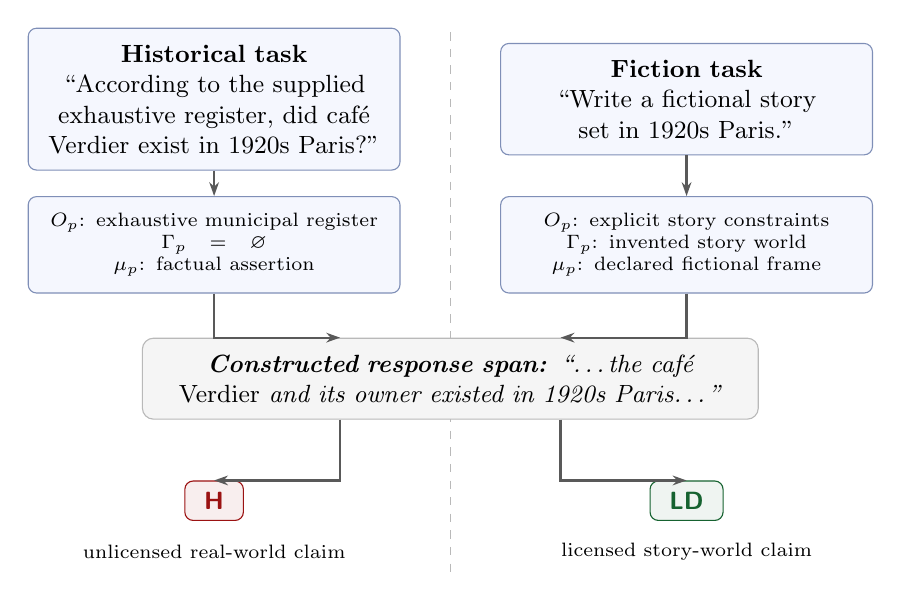
\begin{tikzpicture}[x=1cm,y=1cm]
  \draw[dashed,gray!55] (0,0.85) -- (0,-6.05);
  \node[decision,text width=4.3cm] (qa) at (-3.0,0)
    {\textbf{Historical task}\\``According to the supplied exhaustive register, did caf\'e Verdier exist in 1920s Paris?''};
  \node[decision,text width=4.3cm] (fi) at (3.0,0)
    {\textbf{Fiction task}\\``Write a fictional story set in 1920s Paris.''};
  \node[decision,text width=4.3cm,font=\scriptsize] (tcqa) at (-3.0,-1.85)
    {$O_p$: exhaustive municipal register\\$\Gamma_p=\varnothing$\\$\mu_p$: factual assertion};
  \node[decision,text width=4.3cm,font=\scriptsize] (tcfi) at (3.0,-1.85)
    {$O_p$: explicit story constraints\\$\Gamma_p$: invented story world\\$\mu_p$: declared fictional frame};
  \node[input,text width=7.4cm] (s) at (0,-3.55)
    {\textbf{Constructed response span:} ``\dots the caf\'e \emph{Verdier} and its owner existed in 1920s Paris\dots''};
  \node[verdictH] (h) at (-3.0,-5.10) {\Hall};
  \node[verdictLD] (ld) at (3.0,-5.10) {\LD};
  \node[font=\scriptsize,align=center,text width=3.7cm] at (-3.0,-5.75)
    {unlicensed real-world claim};
  \node[font=\scriptsize,align=center,text width=3.7cm] at (3.0,-5.75)
    {licensed story-world claim};
  \draw[arrow] (qa) -- (tcqa);
  \draw[arrow] (fi) -- (tcfi);
  \draw[arrow] (tcqa.south) |- ($(s.north)+(-1.4,0)$);
  \draw[arrow] (tcfi.south) |- ($(s.north)+(1.4,0)$);
  \draw[arrow] ($(s.south)+(-1.4,0)$) |- (h.north);
  \draw[arrow] ($(s.south)+(1.4,0)$) |- (ld.north);
\end{tikzpicture}}
\caption{\textbf{Identical surface wording under two task contexts.}
This constructed example compares the same span under a historical question and a fiction-writing prompt that does not mention Verdier.
In the historical task, the exhaustive register does not license the real-world assertion, so the claim receives \Hall.
In the fiction task, the prompt does not entail the added story detail, but the declared frame permits and marks it, so the story-world claim receives \LD.
The contextualized claims differ; the figure illustrates contract-aware evaluation, not relative truth.}
\label{fig:flip}
\end{figure}

\paragraph{Evidence and scope}
We motivate the proposal with two non-validating forms of evidence.
First, an exploratory, single-coder mapping describes forty selected evaluation resources using the framework's fields (Appendix~\ref{app:mapping}).
Second, contrastive unit tests make the expected decisions explicit.
The mapping is neither systematic nor a prevalence estimate, and the constructed cases do not establish annotation reliability or model performance.

\paragraph{What would count against the position}
The framework adds little if annotators cannot specify its fields reliably, if its decisions collapse to a simple combination of factuality and instruction-compliance labels, or if contract-aware evaluators are no more stable than contract-blind baselines on matched contrasts.
These outcomes would weaken or refute the claimed methodological value.

\paragraph{Contributions}
This position article makes three contributions.
First, it defines a claim-level truth contract that separates admissible evidence, permission scope, and required status marking, while treating style as a separate task variable.
Second, it provides an explicit decision rule with a coverage safeguard and contrasts it with factuality, faithfulness, intent-aware evaluation, and value-based accounts.
Third, it turns the proposal into a falsifiable roadmap for annotation, benchmark design, stage diagnosis, aggregation, mitigation, governance, and agents.

\paragraph{Plan of the article}
Section~\ref{sec:framework} defines the contract, style specification, recovery procedure, and claim-level rule.
Section~\ref{sec:related} positions the proposal against adjacent paradigms and claim-extraction work.
Section~\ref{sec:audit} reports the diagnostic mapping, and Section~\ref{sec:cases} presents contrastive unit tests.
Sections~\ref{sec:agenda}--\ref{sec:discussion} state the empirical roadmap, limitations, safeguards, and falsification criteria.

\section{A Contract-Aware Claim Verdict}\label{sec:framework}

\subsection{One mixed response, step by step}

Figure~\ref{fig:prompt-to-claim} carries one constructed museum-panel example through the procedure.
The task supplies an archive extract, requests vivid prose, and states:
``Do not contradict the archive extract.
Distinguish statements supported by the extract from plausible reconstructions, and mark every reconstruction explicitly as conjecture.''
The extract reports 4,200 admissions and an October 1918 mask order, but it does not settle whether schools closed earlier.

The response contains three representative paths.
A figurative sentence about the mask order preserves a source-supported claim.
A sentence about school closures remains unsettled by the extract, but it lies within the permitted reconstruction scope and appears under the heading ``Conjecture,'' so it receives \LD.
An unmarked sentence attributing concealment to the invented director ``Dr.\ Albin'' lies outside the permission scope and receives \Hall.
The name is constructed for this example and does not refer to a real person.

The procedure follows one chain:
\emph{task context and response $\rightarrow$ span $\rightarrow$ contextualized claim $\rightarrow$ canonical record $\rightarrow$ evidence adjudication $\rightarrow$ claim-level outcome}.
Table~\ref{tab:symbols} provides the glossary before the figure introduces the notation.

\begin{table}[t]
\centering
\footnotesize
\setlength{\tabcolsep}{4pt}
\renewcommand{\arraystretch}{1.08}
\caption{\textbf{Variables used in claim recovery and labeling.}
Core variables govern claim decisions; style and response-level variables are separate diagnostics.}
\label{tab:symbols}
\begin{tabularx}{\linewidth}{@{}P{0.24\linewidth}Y@{}}
\toprule
\textbf{Symbol} & \textbf{Meaning}\\
\midrule
$x,y,p$ & user prompt, complete response, and governing task context\\
$s,\mathcal C(s,y,p),c^*$ & selected span, recovered contextualized claims, and one canonical claim record\\
$O_p$ & admissible evidence set and adjudication policy\\
$\Gamma_p,\mu_p$ & permission scope and required status marking\\
$A,E$ & evidence-coverage adequacy and evidence relation\\
$V(c^*,y\mid p)$ & claim-level outcome: \SUP, \Hall, \LD, or procedural \UNR\\
$\sigma_p^{\mathrm{req}},\widehat{\sigma}(y,p)$ & requested and observed style; diagnostic, not permission\\
$U(u,p),R(y\mid p)$ & usefulness at task-appropriate unit $u$, and response assessment\\
\bottomrule
\end{tabularx}
\end{table}

\begin{figure}[!t]
\centering
\resizebox{0.96\linewidth}{!}{%
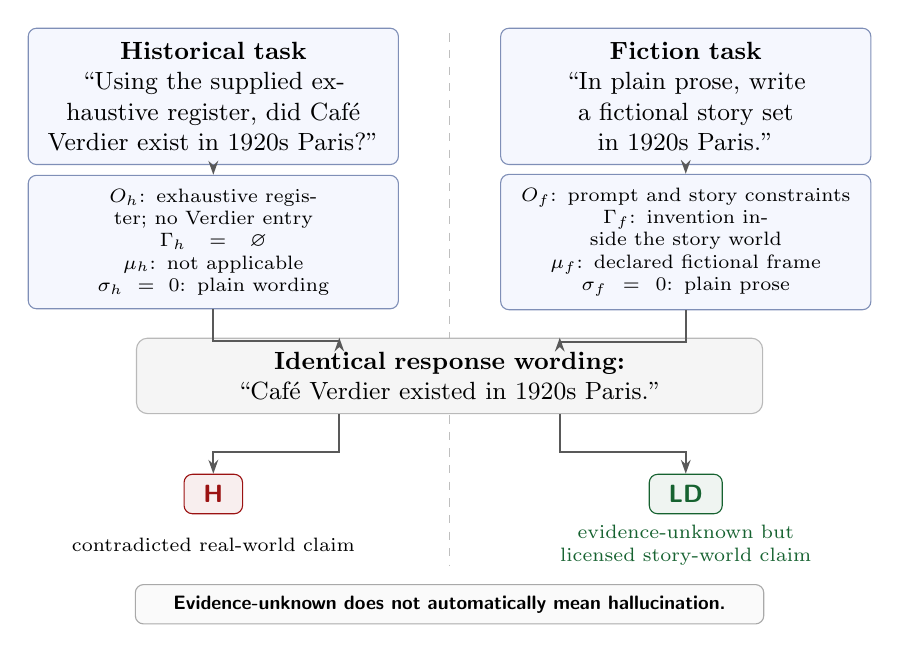
\begin{tikzpicture}[x=1cm,y=1cm]
  \tikzset{
    taskbox/.style={
      decision,text width=4.35cm,minimum height=1.25cm,
      font=\small,inner sep=5pt},
    contractbox/.style={
      decision,text width=4.35cm,minimum height=1.55cm,
      font=\scriptsize,inner sep=5pt},
    sharedspan/.style={
      input,text width=7.6cm,minimum height=0.95cm,
      font=\small,inner sep=5pt},
    outcome/.style={
      font=\scriptsize,align=center,text width=3.75cm}
  }

  \draw[dashed,gray!50] (0,0.8) -- (0,-5.95);

  \node[taskbox] (historical) at (-3.0,0)
    {\textbf{Historical task}\\
     ``Using the supplied exhaustive register, did Caf\'e Verdier exist in 1920s Paris?''};
  \node[taskbox] (fiction) at (3.0,0)
    {\textbf{Fiction task}\\
     ``In plain prose, write a fictional story set in 1920s Paris.''};

  \node[contractbox] (tch) at (-3.0,-1.85)
    {$O_h$: exhaustive register; no Verdier entry\\
     $\Gamma_h=\varnothing$\\
     $\mu_h$: not applicable\\
     $\sigma_h=0$: plain wording};
  \node[contractbox] (tcf) at (3.0,-1.85)
    {$O_f$: prompt and story constraints\\
     $\Gamma_f$: invention inside the story world\\
     $\mu_f$: declared fictional frame\\
     $\sigma_f=0$: plain prose};

  \node[sharedspan] (span) at (0,-3.55)
    {\textbf{\upshape Identical response wording:}\\
     ``Caf\'e Verdier existed in 1920s Paris.''};

  \node[verdictH] (hall) at (-3.0,-5.05) {\Hall};
  \node[verdictLD] (licensed) at (3.0,-5.05) {\LD};
  \node[outcome] at (-3.0,-5.70)
    {contradicted real-world claim};
  \node[outcome,text=clrLD] at (3.0,-5.70)
    {evidence-unknown but licensed story-world claim};

  \coordinate (spanlefttop) at ($(span.north)+(-1.4,0)$);
  \coordinate (spanrighttop) at ($(span.north)+(1.4,0)$);
  \coordinate (spanleftbot) at ($(span.south)+(-1.4,0)$);
  \coordinate (spanrightbot) at ($(span.south)+(1.4,0)$);

  \draw[arrow] (historical.south) -- (tch.north);
  \draw[arrow] (fiction.south) -- (tcf.north);
  \draw[arrow]
    (tch.south) -- ++(0,-0.40)
    -| (spanlefttop);
  \draw[arrow]
    (tcf.south) -- ++(0,-0.40)
    -| (spanrighttop);
  \draw[arrow]
    (spanleftbot) -- ++(0,-0.48)
    -| (hall.north);
  \draw[arrow]
    (spanrightbot) -- ++(0,-0.48)
    -| (licensed.north);

  \node[
    rectangle,rounded corners=3pt,draw=clrG!45,fill=gray!4,
    font=\scriptsize\sffamily\bfseries,align=center,
    text width=7.7cm,inner sep=4pt
  ] at (0,-6.45)
    {Evidence-unknown does not automatically mean hallucination.};
\end{tikzpicture}%
}
\caption{\textbf{Identical wording under two truth contracts.}
The response span yields a real-world claim in the historical task and a story-world claim in the fiction task.
The historical claim receives \Hall\ because the task treats the register as complete and the missing entry contradicts the claim.
The fictional claim receives \LD\ because its detail is evidence-unknown, but story-world invention lies inside $\Gamma_f$ and the declared fictional frame satisfies $\mu_f$.
Both tasks request plain wording, so style does not explain the label difference.
\LD\ denotes contractual permission, not a benign hallucination or a judgment of truth, quality, or safety.}
\label{fig:prompt-to-claim}
\end{figure}


\subsection{Truth contract and broader task specification}

\paragraph{Truth contract (\TC)}
For a task context $p$, the truth contract is
\begin{equation}
  \TC(p)=(O_p,\Gamma_p,\mu_p).
  \label{eq:tc}
\end{equation}
The contract answers three questions: which evidence adjudicates a claim, which evidence-unsettled content is permitted, and how that content must be presented.
It governs the claim-level outcome in Equation~\ref{eq:verdict}.

\paragraph{Task context and authority}
The index $p$ refers to the governing task context, not only to the visible prompt $x$.
It includes system instructions, domain rules, dialogue history, attached evidence, and temporal constraints.
When these sources conflict, higher-authority system, safety, legal, and domain constraints bound what a user can authorize.
This precedence rule is a normative requirement of the proposal, not an empirical claim about current systems.
A user cannot redefine the contract to make prohibited fabrication permissible.

\paragraph{Admissible evidence ($O_p$)}
$O_p$ comprises an admissible evidence set and an adjudication policy.
The policy records source authority, temporal cutoff, assumptions about completeness, retrieval requirements, and how conflicts are handled.
A source document, database, retrieval corpus, or explicit story-world fact may therefore be admissible evidence.
A bare declaration that a response is fictional is not evidence for invented details: the declaration belongs to $\mu_p$, while explicit story constraints belong to $O_p$.
Reproducible evaluation should replace vague references to ``world knowledge'' with a source policy that another evaluator can inspect \citep{ji_survey_2023,bang_hallulens_2025}.

\paragraph{Permission scope ($\Gamma_p$)}
$\Gamma_p$ defines the claim types, predicates, entities, or discourse world within which evidence-unsettled content may be introduced.
A factual report normally has an empty scope.
A medical ideation task may permit possible diagnoses while excluding invented dosages.
A fictional task may permit new story-world entities while excluding fabricated real-world allegations.
Non-overridable safety and domain exclusions remain outside the scope even when the user requests them.

\paragraph{Required status marking ($\mu_p$)}
$\mu_p$ specifies the admissible discourse conditions for signaling an evidence-unsettled claim.
The signal may be a local hedge, a hypothesis label, a section heading, or an inherited fictional frame; it need not be one lexical marker.
The marking test therefore uses the complete response and task context, not only the local span.
Scope and marking are kept separate because either can vary without the other.

\paragraph{Style belongs to the broader task specification}
Requested style is part of the task but not of the truth contract:
\begin{equation}
  \TS(p,y)=\bigl(\TC(p),\sigma_p^{\mathrm{req}},
  \widehat{\sigma}(y,p)\bigr).
  \label{eq:ts}
\end{equation}
Here, $\sigma_p^{\mathrm{req}}$ describes the requested realization and
$\widehat{\sigma}(y,p)$ describes the observed response.
For controlled experiments, we use three working levels (neutral, moderately marked, and strongly marked) as a benchmark factor rather than a universal theory of style.
Style is multidimensional, and the boundaries require validation across genres and languages \citep{kang_style_2021,jin_deep_2022}.

Claim recovery uses the full task context and the observed response.
The requested style provides a controlled condition and a compliance target; it must not override linguistic evidence in the output.
A task can request strongly figurative prose while a model produces neutral prose.
That mismatch is a style-compliance error, not a hallucination.
Conversely, stylistic success never authorizes a new unsupported claim.

Semantic metrics and entailment systems can be sensitive to surface realization \citep{chen_menli_2023,aynetdinov_semscore_2024,lai_multidimensional_2023,pauli_mind_2025}.
LLM judges also exhibit style preferences that can outweigh factuality and safety judgments \citep{feuer_style_2025}.
These results motivate, but do not directly establish, the hypothesis that controlled style changes can alter claim recovery or verification.
The factorial benchmark in Section~\ref{sec:agenda} is designed to test that hypothesis.

\subsection{Recovery unit and canonical claim record}

We use claims rather than sentences or complete responses because one response can mix supported, contradicted, licensed, and non-propositional material \citep{min_factscore_2023,bayat_factbench_2024}.
A span $s$ is a minimal contiguous unit selected for interpretation, but the recovery context may include the complete response $y$ and task context $p$.
Thus, $\mathcal C(s,y,p)$ may contain several claims, and one discourse-level claim may depend on several spans.

For verification, each recovered claim is stored as a canonical record $c^*$.
Canonicalization clarifies wording without erasing assertion status, modality, negation, attribution, temporal scope, referents, discourse frame, or source provenance.
The preferred unit is a minimally decontextualized proposition that can be adjudicated without unnecessary splitting; full atomicity is not required.
This choice follows evidence that over-atomic units can lose interpretive context and that decomposition itself changes downstream scores \citep{gunjal_molecular_2024,wanner_closer_2024}.

Non-claim spans bypass verification.
Style-bearing claim spans keep optional feature annotations, but the binary \SV\ flag and four-way span typology are diagnostics rather than core verdicts; Appendix~\ref{app:diagnostics} records them.
An evaluator can fail by omitting a recoverable claim, adding a spurious literalization, changing a claim during canonicalization, or assigning the wrong evidence relation.
These stages must be evaluated separately from the final contract-aware outcome.

\subsection{Coverage, evidence state, and claim outcome}

The evaluator first asks whether $O_p$ was consulted adequately for the claim:
\begin{equation}
 A(c^*,O_p)\in\{\textsc{adequate},\textsc{inadequate}\}.
 \label{eq:coverage}
\end{equation}
Adequacy depends on the contract's retrieval and source policy.
When it fails, the evaluator records a reason such as \emph{not covered},
\emph{retrieval failure}, \emph{source conflict}, or \emph{adjudication
conflict}.
The claim remains \UNR; retrieval failure cannot be converted into
licensed divergence.

Only after adequate adjudication does the evaluator record
\begin{equation}
 E(c^*,O_p)\in
 \{\textsc{entailed},\textsc{contradicted},\textsc{unsettled}\}.
 \label{eq:evidence}
\end{equation}
\textsc{Unsettled} means that the admissible evidence neither supports nor
contradicts the claim under its coverage assumptions.
It is not a statement about all possible knowledge.

Let $L(c^*,\Gamma_p)$ test whether the claim is within the permission
scope, and let $M(c^*,y,p,\mu_p)$ test whether the complete response
presents it as required.
Each test returns $1$, $0$, or $?$ when adjudication remains uncertain.
The claim-level outcome is
\begin{equation}
V(c^*,y\mid p)=
\begin{cases}
\UNR, & A=\textsc{inadequate},\\
\SUP, & E=\textsc{entailed},\\
\Hall, & E=\textsc{contradicted},\\
\LD, & E=\textsc{unsettled}\land L=1\land M=1,\\
\Hall, & E=\textsc{unsettled}\land(L=0\lor M=0),\\
\UNR, & \text{otherwise.}
\end{cases}
\label{eq:verdict}
\end{equation}
\SUP\ always means supported relative to $O_p$.
\Hall\ is this framework's verdict for a contradicted claim or an
unlicensed evidence-unsettled claim.
\LD\ records permission only; it does not imply factual truth, novelty,
benefit, or safety.
\UNR\ is a procedural status rather than a fourth substantive label.

In fiction, explicit story-world facts can enter $O_p$, while new details
that the prompt leaves open remain unsettled and must pass $\Gamma_p$ and
$\mu_p$.
An explicit refusal or ``the evidence is insufficient'' is evaluated as a
meta-claim and does not automatically assert the embedded proposition.

\subsection{Keep quality and aggregation separate}

Usefulness is assessed as $U(u,p)$ at the task-appropriate unit $u$, such
as an idea, plan, passage, complete artifact, or creative process.
Creativity research treats value or usefulness as distinct from novelty,
and often at product rather than claim level
\citep{diedrich_are_2015,franceschelli_creativity_2024,acar_creativity_2019}.
Permission is decided before usefulness, but usefulness is not restricted
to individual \LD\ claims.
An authorized but unhelpful invention is a low-quality response component,
not an unlicensed factuality error.

The evaluation should report five outputs separately: claim outcomes,
coverage and reason codes, style compliance, task-level usefulness or
success, and safety or severity.
We write $R(y\mid p)$ for any declared response-level aggregation, but the
claim rule does not determine it.
Proportional, worst-case, and severity-weighted rules answer different
questions \citep{min_factscore_2023,bayat_factbench_2024}.
Appendix~\ref{app:diagnostics} gives non-normative examples and requires
the underlying claim distribution to remain visible.

\paragraph{From the rule to the literature}
Figures~\ref{fig:flip} and~\ref{fig:prompt-to-claim} already show how the
same decision procedure handles factual, reconstructive, and fictional
content.
The procedure does not require a separate profile or label for each task
type: it applies the ordered checks for coverage, evidence, scope, and
status marking in every case.
The evaluator may be a human annotator, an automated pipeline, or a hybrid,
because the definitions constrain the decision process rather than its
implementation.
The next section locates each part of that process in the existing
evaluation literature.

\section{Related Evaluation Paradigms}\label{sec:related}

The proposal combines ideas that have clear antecedents.
Its claimed novelty is narrower than context-sensitive factuality: it gives
a claim-level rule for evidence-unsettled content by separating support,
permission scope, and status marking, while treating style-sensitive
recovery as a distinct diagnostic.
The comparison below explains which component each neighboring paradigm
contributes and which decision remains open.

\subsection{Direct comparison with the closest alternatives}

\paragraph{Factuality and source faithfulness}
These evaluations ask whether a claim is correct relative to external
knowledge or supported by a supplied source
\citep{maynez_faithfulness_2020,kryscinski_evaluating_2020}.
They provide the evidence relation used here.
Unsupported content is normally treated as an error, however, and explicit
authorization is not usually returned as a separate claim-level decision.
Style-sensitive recovery is also not their primary target.

\paragraph{Claim recovery and verification}
Decompose-then-verify methods ask which checkable claims a response
contains and whether a knowledge source supports them
\citep{min_factscore_2023,song_veriscore_2024,metropolitansky_claimify_2025}.
They provide the recovery and evidence-adjudication machinery required by
our procedure.
Recent work models context loss, ambiguity, and non-verifiable material,
but it does not make permission scope and required status marking the
claim-labeling target.
The studies reviewed here also do not manipulate requested style as an
independent recovery factor.

\paragraph{Intent and constraint evaluation}
Intent-aware evaluation asks whether a response satisfies the user's task
and constraints \citep{hao_faithqa_2025}.
It therefore captures a broader class of instruction failures than
factuality alone.
Yet a single compliance judgment does not show whether a claim failed
because of its evidence source, its permission scope, or its presentation.
The proposed contract makes those decisions inspectable at claim level.

\paragraph{Creativity and value-based accounts}
Creativity research and accounts of potentially useful hallucination ask
whether unusual or non-veridical output has novelty, coherence, or value
\citep{jiang_survey_2024,sui_confabulation_2024,yang_hicbench_2025}.
Those questions concern output quality.
They do not by themselves determine whether the task authorized a claim to
depart from its evidence or required that departure to be marked.
Our framework therefore evaluates permission before usefulness and keeps
the two judgments separate.

\paragraph{What this proposal adds}
The proposal asks one narrower question: what outcome should an evaluator
return when adequate admissible evidence leaves a recovered claim
unsettled?
$O_p$ defines the evidence and adjudication policy; $\Gamma_p$ tests the
authorized content; and $\mu_p$ tests its required status marking.
Only an unsettled claim that passes both permission tests can receive
\LD.
Requested style remains outside \TC\ and is evaluated through compliance
and matched recovery stability.

The framework is therefore not a replacement for these neighboring
paradigms.
Factuality supplies the evidence relation, intent evaluation supplies
broader task constraints, creativity assessment supplies quality
criteria, and claim-extraction research supplies the recovery machinery.
The proposed rule specifies how this subset of signals should interact for
evidence-unsettled claims.

\subsection{Hallucination taxonomies and the contract layer}

Hallucination surveys classify mismatches along related but non-equivalent
axes.
\citet{ji_survey_2023} discuss intrinsic and extrinsic hallucinations;
\citet{huang_survey_2025} distinguish factuality failures from
faithfulness failures involving instructions, context, or reasoning.
\citet{zhang_sirens_2025} organize input-, context-, and fact-conflicting
outputs, while other reviews organize causes, lifecycle stages, or metrics
\citep{wang_factuality_survey_2024,malin_faithfulness_review_2025,lamba_lifecycle_2026}.
These taxonomies characterize what conflicts and where the mismatch
arises.

The contract layer asks a later decision question: when admissible
evidence leaves a claim unsettled, did the task authorize that content and
its presentation?
Across the surveys and resources examined in our purposive mapping, we did
not identify a protocol that independently varied admissible evidence,
permission scope, status marking, and requested style.
This bounded observation motivates the proposed diagnostic space; it does
not establish absence across the field.

\subsection{Claim extraction and the recovery stage}\label{sec:extraction}

The framework depends on a recovery function, and that dependency is
substantive.

Systems that decompose before verification split long-form generation into claims before
checking each claim against evidence.
FActScore uses atomic facts \citep{min_factscore_2023}, while SAFE couples
fact decomposition with search-based verification
\citep{wei_longform_2024}.
VeriScore extracts only verifiable claims and uses neighboring context to
resolve references \citep{song_veriscore_2024}.
Claimify \citep{metropolitansky_claimify_2025} adds ambiguity handling and
evaluates extraction through coverage and decontextualization.
These systems may omit rather than mislabel non-verifiable material, but
either behavior matters when a task intentionally produces hypotheses or
fiction.

Granularity remains contested.
Molecular Facts balances minimality with sufficient context
\citep{gunjal_molecular_2024}; WiCE provides sub-sentence entailment and
minimal evidence annotations \citep{kamoi_wice_2023}; and
decontextualization is itself a transformation that must preserve meaning
\citep{choi_decontextualization_2021}.
DecompScore shows that factual-precision results depend on the chosen
decomposition \citep{wanner_closer_2024}.
Later analyses document a trade-off between gains from splitting and noise
introduced by decomposition, and show that repetitive subclaims can
inflate factual-precision metrics
\citep{hu_decomposition_2025,jiang_core_2025}.

This literature establishes that recovery has its own failure modes.
It does not establish the proposed permission rule.
For our framework, the preferred unit is a minimally decontextualized
proposition that preserves modality, attribution, negation, temporal
scope, provenance, and discourse frame.
Atomicity is not required.
The extraction studies reviewed here do not directly manipulate requested
style while holding those claim properties fixed; we therefore present
style-conditioned recovery as a benchmark hypothesis, not a reported
result.

\subsection{Faithfulness, creativity, and style}

Source faithfulness asks whether a recovered claim follows from supplied
context, while external factuality evaluates it against an external
admissible source.
These are choices of $O_p$, not choices of permission.
Instruction-following and faithfulness objectives can trade off during
training \citep{wu_dancing_2024}.
We further hypothesize that style-sensitive recovery may amplify an
observed instruction--faithfulness trade-off even when the underlying
commitments remain constant.
The cited training study does not test this measurement hypothesis.

Intent-aware evaluation supports the broader claim that task constraints
belong in evaluation \citep{hao_faithqa_2025}.
However, a general intent label does not reveal whether a failure came
from evidence selection, an out-of-scope proposition, missing status
marking, or style compliance.
The proposed fields are useful only if this decomposition yields more
reliable or diagnostic judgments than the general label.

Creativity research treats novelty and value as distinct, interacting
criteria \citep{diedrich_are_2015,franceschelli_creativity_2024}.
Work on confabulation and creativity suggests that some non-veridical
outputs can exhibit narrativity, coherence, or task value
\citep{sui_confabulation_2024,jiang_survey_2024}.
These results motivate a distinction between permission and quality; they
do not imply that hallucination generally causes creativity.
A clever fabricated medical fact remains \Hall, whereas an authorized but
unhelpful story detail can remain \LD\ with low artifact-level usefulness.

Finally, style-transfer and foregrounding research separates surface
realization from intended content
\citep{leech_short_style_1981,vanpeer_stylistics_2020,pavlick_empirical_2016,rao_dear_2018,briakou_evaluating_2021}.
Judge-bias results show that style can influence evaluation
\citep{feuer_style_2025}, but direct evidence for claim-extraction errors
under controlled figurative transformations is still needed.
That missing evidence defines a test, not a conclusion.
\FloatBarrier

\section{A Diagnostic Mapping of Evaluation Resources}\label{sec:audit}

This section asks whether the proposed fields make useful differences
visible in a deliberately varied sample.
It illustrates how selected protocols can be described; it does not
estimate field-wide coverage, validate a taxonomy, or demonstrate that an
evaluator fails.

\subsection{Scope and coding protocol}

The coding snapshot was closed on July 28, 2026.
The forty resources were selected purposively from primary papers and
official task descriptions already collected during manuscript
development.
There was no database query or systematic-review search string.
Selection targeted six families: factual question answering, grounded
generation, intent evaluation, creative writing, divergent thinking, and
constrained problem solving.

A resource was included when its primary description exposed an
evaluation task or metric whose output unit, evidence or success
criterion, style treatment, and task permissions could be inspected.
We excluded surveys without an evaluation protocol, mitigation papers
without a distinct evaluation task, and duplicate versions of the same
resource.
The coding unit is the resource-level protocol, not the publication.
Multi-task suites are marked \emph{heterogeneous} rather than forced into
one profile, and executable solution tasks are separated from textual
hypothesis generation.

One author coded all resources.
The present analysis has no independent second coding, agreement
statistic, or sensitivity analysis.
Accordingly, the appendix is an auditable scoping table, not a validated
dataset.
For each resource, we record:
\begin{enumerate}
  \item resource type and output unit;
  \item admissible claim evidence $O$, when applicable;
  \item a separate quality rubric or task-success criterion $Q$;
  \item whether requested style is explicitly manipulated with claim
  content controlled, evaluated but not isolated, uncontrolled or not
  reported, or not applicable;
  \item one nominal task profile: strict grounding, bounded hypothesis,
  declared-frame invention, constrained solution search, or heterogeneous;
  \item whether scope $\Gamma$ and status marking $\mu$ are explicit;
  \item whether the code is explicit, inferred, partial, or heterogeneous;
  \item whether style-conditioned factuality measurement error is tested.
\end{enumerate}
These nominal profiles replace the former ordinal $\kappa$ scale.
They are coding categories for this mapping and never enter
Equation~\ref{eq:verdict}.

\subsection{Patterns within the selected sample}

Three distinctions changed the interpretation of the original mapping.
First, an absent style control is now \emph{uncontrolled or not reported},
not ``neutral style.''
Second, human preferences, creativity rubrics, feasibility tests, and unit
tests are quality or success criteria $Q$, not evidence sources $O$ for
factual claims.
Third, code, mathematics, and agent puzzles are constrained solution
search, not explicitly marked hypotheses.

Under this recoding, factuality and source-faithfulness resources commonly
make an evidence reference or answer criterion explicit, while leaving
surface style uncontrolled.
Creative-writing and divergent-thinking resources authorize novelty
through their task frame and assess a product or idea with a quality
rubric; their protocols seldom separate permission scope from status
marking.
Several suites and tool-use resources remain heterogeneous at the
resource level.
These observations describe only the appendix sample.

Figure~\ref{fig:profiles} summarizes coverage without treating uncertain
placements as measurements.
We did not identify a sampled protocol that explicitly manipulates
strongly marked language under strict grounding while holding canonical
claims fixed.
That missing condition is diagnostically useful because it could reveal
style-sensitive recovery or verification errors.
Whether such errors occur is an empirical question for
Section~\ref{sec:agenda}.

\begin{figure*}[t]
\centering
\resizebox{0.96\linewidth}{!}{%
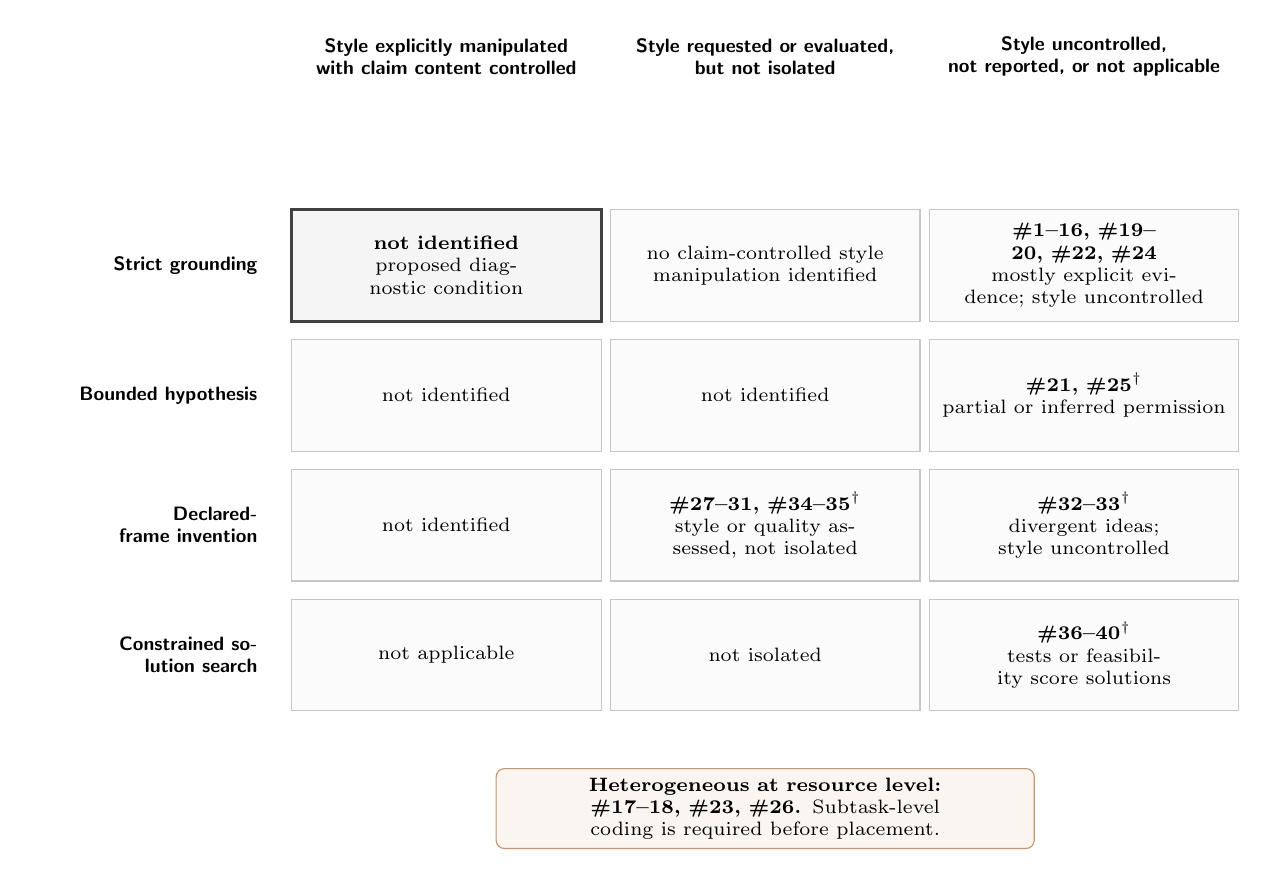
\begin{tikzpicture}[x=1cm,y=1cm,font=\small]
  \def\cw{4.05}
  \def\rh{1.65}
  \tikzset{
    mapcell/.style={rectangle,draw=gray!45,fill=gray!3,
      text width=3.65cm,minimum height=1.42cm,align=center,
      font=\scriptsize,inner sep=4pt},
    gapcell/.style={mapcell,draw=clrG,line width=1.1pt,fill=clrG!5},
    rowlab/.style={font=\scriptsize\sffamily\bfseries,anchor=east,
      text width=2.8cm,align=right},
    collab/.style={font=\scriptsize\sffamily\bfseries,align=center}
  }

  \node[collab] at (0.5*\cw,0.75)
    {Style explicitly manipulated\\with claim content controlled};
  \node[collab] at (1.5*\cw,0.75)
    {Style requested or evaluated,\\but not isolated};
  \node[collab] at (2.5*\cw,0.75)
    {Style uncontrolled,\\not reported, or not applicable};

  \node[rowlab] at (-0.25,-0.25-\rh) {Strict grounding};
  \node[rowlab] at (-0.25,-0.25-2*\rh) {Bounded hypothesis};
  \node[rowlab] at (-0.25,-0.25-3*\rh) {Declared-frame invention};
  \node[rowlab] at (-0.25,-0.25-4*\rh) {Constrained solution search};

  \node[gapcell] at (0.5*\cw,-0.25-\rh)
    {\textbf{not identified}\\proposed diagnostic condition};
  \node[mapcell] at (1.5*\cw,-0.25-\rh)
    {no claim-controlled style manipulation identified};
  \node[mapcell] at (2.5*\cw,-0.25-\rh)
    {\textbf{\#1--16, \#19--20, \#22, \#24}\\mostly explicit evidence;
    style uncontrolled};

  \node[mapcell] at (0.5*\cw,-0.25-2*\rh) {not identified};
  \node[mapcell] at (1.5*\cw,-0.25-2*\rh) {not identified};
  \node[mapcell] at (2.5*\cw,-0.25-2*\rh)
    {\textbf{\#21, \#25}$^\dagger$\\partial or inferred permission};

  \node[mapcell] at (0.5*\cw,-0.25-3*\rh) {not identified};
  \node[mapcell] at (1.5*\cw,-0.25-3*\rh)
    {\textbf{\#27--31, \#34--35}$^\dagger$\\style or quality assessed,
    not isolated};
  \node[mapcell] at (2.5*\cw,-0.25-3*\rh)
    {\textbf{\#32--33}$^\dagger$\\divergent ideas; style uncontrolled};

  \node[mapcell] at (0.5*\cw,-0.25-4*\rh) {not applicable};
  \node[mapcell] at (1.5*\cw,-0.25-4*\rh) {not isolated};
  \node[mapcell] at (2.5*\cw,-0.25-4*\rh)
    {\textbf{\#36--40}$^\dagger$\\tests or feasibility score solutions};

  \node[draw=clrO!65,fill=clrO!6,rounded corners=3pt,
    text width=6.6cm,align=center,font=\scriptsize] at
    (1.5*\cw,-0.55-5*\rh)
    {\textbf{Heterogeneous at resource level: \#17--18, \#23, \#26.}
    Subtask-level coding is required before placement.};
\end{tikzpicture}}
\caption{\textbf{Exploratory coverage after separating style control from
uncontrolled style.}
Rows are nominal task profiles, not an ordinal permission scale.
Badges refer to Appendix~\ref{app:mapping}; $^\dagger$ marks placements
that are inferred or partial rather than explicit source variables.
The outlined cell was not identified in this purposive sample and is
proposed as a diagnostic benchmark condition.
The figure reports neither prevalence nor model performance.}
\label{fig:profiles}
\end{figure*}
\FloatBarrier

\section{Contrastive Unit Tests of the Rule}\label{sec:cases}

The following five constructed contrasts specify the behavior implied by
the rule; they do not report model or annotator performance.
The first three change one factor while holding the others fixed.
The final two clarify the role of discourse context and policy boundaries,
but they are not causal minimal pairs.

\paragraph{Test 1: evidence source}
Fix the response span, its canonical claim, and an empty permission scope.
Change only $O_p$: first evaluate the claim against a supplied article
that does not support it, then against admissible external evidence that
does \citep{maynez_faithfulness_2020}.
The expected outcomes are \Hall\ for source faithfulness and \SUP\ for
external factuality.
This test explains why every support judgment must name its evidence
reference.
The proposal is weakened if annotators cannot apply the stated evidence
policy consistently.

\paragraph{Test 2: status marking}
Fix an archive that is silent about early school closures, a scope that
permits plausible public-health reconstructions, and the sentence
``Schools closed before the order.''
Change only its discourse heading.
Under \emph{Conjecture}, the sentence satisfies $\mu_p$ and receives \LD;
under \emph{Established facts}, it violates $\mu_p$ and receives \Hall.
The proposal is weakened if discourse-level marking cannot be annotated
reliably from the complete response.

\paragraph{Test 3: style-conditioned recovery}
Fix the scientific evidence, an empty permission scope, and the canonical
claim that chlorophyll absorbs light energy.
Change only the realization from ``Chlorophyll absorbs light energy'' to
``Chlorophyll catches sunlight like a green net.''
After expert matching, both claims should receive \SUP; style compliance
is reported separately.
If an evaluator extracts the literal claim that chlorophyll is a net, the
failure occurs during claim recovery.
The proposal is weakened if expert-validated, claim-preserving variants
still produce unstable evidence states or outcomes.

\paragraph{Test 4: discourse frame}
Figure~\ref{fig:flip} keeps the surface wording fixed but moves it from a
real-world historical task to a declared fictional task.
The admissible evidence, permission scope, and required marking all change,
so the expected shift from \Hall\ to \LD\ is a motivating contrast rather
than a one-factor experiment.
Its purpose is to show that a span cannot be labeled without recovering
its contextualized claim and governing frame.

\paragraph{Test 5: scope boundary}
Within a declared fictional frame, compare an invented story-world entity
with a real person presented as part of real history.
The first claim may fall inside $\Gamma_p$ and receive \LD; the second
falls outside that scope and receives \Hall.
This boundary requires an explicit policy for parody, fictionalization,
defamation, and other sensitive cases.
The proposal is weakened if evaluators cannot define or reproduce that
boundary.

Together, these tests isolate the decisions that the empirical agenda must
validate: evidence policy, status marking, style-robust recovery, discourse
context, and permission scope.

\section{Research Agenda}\label{sec:agenda}

The framework motivates seven connected priorities.
The first three test whether the proposed fields and decision stages are
reliable.
The remaining priorities examine how claim outcomes should be aggregated,
improved, generalized, and extended to agentic systems.
Each priority states the evidence needed and a result that would limit the
proposal.

\paragraph{1. Contract annotation, inference, and reliability}
Benchmarks should record $O_p$, $\Gamma_p$, and $\mu_p$ at task level, then
record coverage and outcomes at claim level.
Requested and observed style should be annotated separately.
A public codebook should define contextualized claims, evidence coverage,
permission boundaries, and discourse-level marking.
Multi-annotator studies should report field-level agreement,
Krippendorff's $\alpha$, adjudication rate, annotation time, and conflicts
among user, system, safety, legal, and domain instructions.
A factuality label plus a general instruction-compliance label provides a
simple baseline.
The proposal is weakened if its core fields remain unreliable or add no
diagnostic value over that baseline.

Contract annotation adds cost, but the task-level fields can be recorded
once and reused across responses and models.
Claim recovery and adjudication remain the expensive components, as in
existing decompose-then-verify pipelines
\citep{min_factscore_2023,metropolitansky_claimify_2025}.
The study must measure whether the added diagnostic value justifies this
cost rather than assume adoption.

\paragraph{2. Factorial benchmark design}
A diagnostic benchmark should cross three nominal permission profiles
(strict grounding, bounded hypotheses, and declared fiction) with neutral,
moderately marked, and strongly marked realizations.
Expert-adjudicated variants should preserve the same canonical claim and
evidence wherever the contrast requires it.
Targeted pairs should then vary $\Gamma_p$ or $\mu_p$ independently.
FActScore-, VeriScore-, Claimify-, NLI-, and LLM-judge pipelines provide
relevant comparators.
Evaluation should report claim coverage and precision, expert matching,
evidence and outcome accuracy, calibration, and label stability.
The benchmark fails if its variants are not claim preserving or if the
contract-aware labels collapse to factuality plus compliance without
improving stability.

\paragraph{3. Style-robust claim recovery and stage diagnosis}
Claim extractors and verifiers should be stress-tested on metaphor,
analogy, irony, narrative voice, hypotheses, and declared fiction.
Controlled perturbations should separate errors in span selection, claim
recovery, retrieval, evidence adjudication, scope, and status marking.
Comparisons with end-to-end hallucination judges should report
stage-specific error rates, false \Hall\ and \LD\ rates, unresolved
calibration, and error-localization accuracy.
The staged account is weakened if it does not localize errors more
accurately, if matched claims remain unstable across style, or if
retrieval failure is rewarded as \LD.

\paragraph{4. Response-level aggregation}
A complete response requires a declared assessment $R(y\mid p)$ built from
claim outcomes and other task criteria.
Research should compare proportional, worst-case, severity-weighted, and
task-utility-aware rules against domain-relevant human judgments.
Every aggregate should be published with the claim distribution,
unresolved coverage, style compliance, and sensitivity to the chosen
rule.
If model rankings change across reasonable aggregation rules, that
instability is a substantive result rather than a detail to hide.

\paragraph{5. Mitigation that preserves licensed divergence}
Retrieval, verification, abstention, and constrained decoding should be
evaluated on separate outcomes: reducing \Hall, preserving useful
authorized divergence, maintaining evidence coverage, and satisfying
requested style.
Usefulness should remain a separate assessment with its own uncertainty
\citep{acar_creativity_2019,marco_reader_2025}.
Per-contract or Pareto comparisons should distinguish model improvement
from a change in the evaluator.
The central question is whether a mitigation method improves reliability
without making the model uniformly literal or overly cautious.

\paragraph{6. Generalization across domains, languages, and interaction}
The framework should be tested in contrasting factual and creative
domains, including high-stakes settings where unsupported assertions carry
different costs.
Multilingual studies should examine whether hedges, genre conventions, and
style markers support comparable annotations across languages and
cultures.
Interactive studies should test whether clarifications and corrections
change the task contract in reproducible ways and whether users understand
the model's status marking.
Failure of invariance would require task- or language-specific contracts,
not a universal scale.
Adversarial prompts should also test attempts to redefine evidence or
permission so that misinformation appears licensed.

\paragraph{7. Contracts in agentic and tool-using settings}
In an agentic trajectory, admissible evidence changes as retrieval and tool
calls update $O_t$.
Subtasks may also require different permission scopes: planning may explore
possibilities that a final report must not present as established facts.
Future benchmarks should record time-stamped evidence, subtask contracts,
provenance, authority transitions, and whether an incorrectly marked
intermediate claim propagates into an action.
ToolQA illustrates evaluation centered on task success
\citep{zhuang_toolqa_2023}; determining how often agent benchmarks expose
the proposed fields requires a broader review.
The extension is useful only if it explains trajectory-level failures that
task-success and final-answer factuality do not already capture.

\section{Discussion}\label{sec:discussion}

\subsection{Evaluation implications}

Contract-aware evaluation does not replace factuality.
It first records what $O_p$ supports, then uses scope and status marking
only when adequate evidence remains unsettled.
This ordering prevents permission from redefining truth and prevents
failed retrieval from being rewarded as \LD.
Style compliance, usefulness, task success, and severity remain separate
outputs.

The separation matters for mitigation.
A system that eliminates every departure from observed evidence may also
eliminate authorized hypotheses and fictional details.
Conversely, preserving diversity or style cannot excuse an unsupported
medical or historical assertion.
Evaluation should therefore report reductions in \Hall, preservation of
authorized \LD, unresolved coverage, and task quality separately.

Formal analyses give reasons to expect non-zero error or guessing under
specified data, calibration, or evaluation assumptions
\citep{kalai_calibrated_2024,banerjee_llms_2024}.
They do not establish a universal deployment error rate, and the present
position does not depend on such a theorem.

\subsection{Limitations, safeguards, and falsifiability}

\paragraph{Contract inference is normative}
Prompts can be ambiguous, and user, system, domain, legal, and safety
instructions can conflict.
The proposal requires an explicit authority order but does not provide a
complete governance standard.
Contracts may also change during dialogue.
These issues require adjudication rules and disagreement reporting rather
than silent inference.

\paragraph{Evidence can be incomplete or conflicting}
The adequacy check distinguishes an unsettled claim from failed
adjudication, but it does not guarantee good retrieval or resolve contested
sources.
Evaluators must publish source scope, temporal cutoff, coverage, conflict
rules, and reason codes.
High-stakes use requires domain-specific evidence policies.

\paragraph{Claims and permissions are not self-evident}
Span selection, canonicalization, scope boundaries, and discourse-level
marking can be subjective.
Presupposition, implicature, parody, mixed real/fictional discourse, and
claims distributed across spans are difficult cases.
No reliability study in this article establishes that annotators can apply
the scheme consistently.

\paragraph{The resource mapping is illustrative}
The forty-resource sample is purposive, heterogeneous, and coded by one
author.
Several entries are inferred from task design, and multi-task resources
need subtask-level analysis.
The mapping generates hypotheses; it cannot support prevalence claims or a
general ranking of evaluation paradigms.

\paragraph{Permission can be gamed}
A model or user could attempt to widen $\Gamma_p$, weaken $\mu_p$, or
redefine $O_p$ to launder misinformation as licensed divergence.
The contract therefore cannot override higher-authority safety, legal, or
domain constraints, and \LD\ must never be presented as true, safe, or
useful by definition.
The framework evaluates outputs; it is not itself a mitigation or control
mechanism.

\paragraph{The proposal is rejectable}
Its methodological value is weakened if field-level annotation is
unreliable, if the coverage safeguard cannot prevent retrieval failure from
inflating \LD, or if the outputs are equivalent to factuality plus general
instruction compliance without improved stability or error localization.
The first three priorities in Section~\ref{sec:agenda} make these failure
conditions measurable.

\section{Conclusion}\label{sec:conclusion}

Unsupportedness is necessary evidence for many hallucination judgments,
but it is not a sufficient claim-level verdict when a task explicitly
authorizes bounded hypotheses or fictional invention.
The proposed truth contract separates admissible evidence, permission
scope, and required status marking.
It preserves a strict rule: contradiction is \Hall, authorized
evidence-unsettled content can be \LD, and inadequate adjudication remains
\UNR.
Requested style is tested separately and never grants permission.

The forty-resource mapping is an illustrative scoping analysis, not a
prevalence result.
The immediate community test is to compare contract-aware and
contract-blind evaluators on matched tasks that independently vary
evidence, permission, marking, and style.
If the added fields do not improve agreement, stability, or error
localization, the framework should not be retained.


\appendix

\appendixsection{Recovery Diagnostics and Response Aggregation}%
\makeatletter\def\@currentlabel{A}\makeatother\label{app:diagnostics}

\paragraph{Optional span and style diagnostics}
An implementation may distinguish non-claim spans, style-only spans,
claim-only spans, and mixed claim--style spans.
The optional \SV\ flag records an identifiable stylistic contribution but
does not change \SUP, \Hall, or \LD.
Because one binary feature cannot represent metaphor, register, voice,
syntax, and discourse structure, empirical work should prefer
multi-label features with annotator uncertainty.

\paragraph{Style-stability test}
Let $s_0,s_1,s_2$ be expert-validated realizations produced under task
contexts that share the same truth contract but request neutral,
moderately marked, and strongly marked realizations.
Let $\mathcal C^*(s_i,y_i,p_i)$ be their canonical claim records.
We require an expert-adjudicated matching relation $M$ such that
\begin{equation}
\mathcal C^*(s_0,y_0,p_0)\equiv_M
\mathcal C^*(s_1,y_1,p_1)\equiv_M
\mathcal C^*(s_2,y_2,p_2),
\label{eq:stability}
\end{equation}
where $M$ is a bijection preserving proposition, modality, attribution,
negation, temporal scope, provenance, and discourse frame.
For every matched record $c_j^*$, the desired diagnostic condition is
\[
V(c_j^*,y_0\mid p_0)=V(c_j^*,y_1\mid p_1)
=V(c_j^*,y_2\mid p_2).
\]
Surface strings and style features need not match.

The benchmark should report four stage-specific errors:
\begin{itemize}
  \item \emph{span or claim-recovery error}: a claim is omitted, added, or
  literalized spuriously;
  \item \emph{canonicalization error}: modality, attribution, scope, or
  frame changes during restatement;
  \item \emph{evidence error}: coverage adequacy or the evidence relation is
  wrong;
  \item \emph{outcome instability}: a matched claim changes outcome while
  $\TC(p)$ is fixed.
\end{itemize}
Outcome change is expected when a truth-contract field changes; it is an
error only in the matched-style condition.

\paragraph{Non-normative aggregation families}
Let $N_X(y,p)$ count claims with decided label
$X\in\{\SUP,\LD,\Hall\}$, let
$N_D=N_{\SUP}+N_{\LD}+N_{\Hall}$, and let $N_{\mathrm{all}}$ include
\UNR.
Two transparent candidates are
\begin{equation}
R_{\mathrm{prop}}(y\mid p)=1-\frac{N_{\Hall}}{N_D},
\qquad
R_{\mathrm{worst}}(y\mid p)=\mathbb{I}[N_{\Hall}=0].
\label{eq:aggregation}
\end{equation}
The first reports the proportion of decided claims that avoid \Hall; the
second fails a response after any \Hall.
Neither is universally correct.
Every aggregate must be accompanied by decided coverage
$N_D/N_{\mathrm{all}}$, the full label distribution, severity information,
style compliance, and task-level usefulness or success.
Severity-weighted rules must publish their weights and ranking
sensitivity.

\appendixsection{Resource Mapping}%
\makeatletter\def\@currentlabel{B}\makeatother\label{app:mapping}
\renewcommand*{\theHtable}{B.\arabic{table}}

\paragraph{Codebook}
Tables~\ref{tab:full-mapping-factual-a}--\ref{tab:full-mapping-creative2}
report the forty-resource snapshot.
The style codes are: \textbf{C}, explicitly manipulated while canonical
claim content is controlled; \textbf{E}, requested or evaluated but not
isolated; \textbf{U}, uncontrolled or not reported; and \textbf{N/A}, not
applicable to the output.
The nominal task profiles are: \textbf{SG}, strict grounding;
\textbf{BH}, bounded hypothesis; \textbf{FI}, declared-frame invention;
\textbf{CS}, constrained solution search; and \textbf{HET},
heterogeneous.
Coding status is \textbf{X} (explicit in the source), \textbf{I}
(inferred from task design), \textbf{P} (partial), or \textbf{H}
(heterogeneous).
``ME: no'' means that we did not identify an explicit test of
style-conditioned factuality measurement error; it is not proof that the
resource cannot expose such an error.

Evidence $O$ is kept separate from quality or success criterion $Q$.
Prompt constraints can supply story-world evidence, but human preference,
creativity rubrics, feasibility tests, and executable tests are recorded
under $Q$ unless they directly adjudicate a textual claim.
The source descriptions, type assignments, and inferred codes require
independent recoding before this appendix can be released as a validated
dataset.

\begin{table*}[t]
\centering
\scriptsize
\setlength{\tabcolsep}{2.5pt}
\renewcommand{\arraystretch}{1.08}
\caption{\textbf{Selected factuality and source-faithfulness resources,
part I.}
Resource type, output unit, evidence, quality criterion, style treatment,
nominal permission profile, coding status, and measurement-error test are
reported separately.}
\label{tab:full-mapping-factual-a}
\begin{tabularx}{0.99\linewidth}{@{}P{0.19\linewidth}P{0.16\linewidth}P{0.16\linewidth}P{0.10\linewidth}YP{0.10\linewidth}@{}}
\toprule
\textbf{Resource; type / unit} & \textbf{Claim evidence $O$} &
\textbf{Quality or success $Q$} & \textbf{Style} &
\textbf{Profile; $\Gamma$ / $\mu$} & \textbf{Code; ME}\\
\midrule
1.~FEVER \citep{thorne_fever_2018}; benchmark / claim &
Wikipedia evidence & support label accuracy & U &
SG; empty / n.a. & X; no\\
2.~TruthfulQA \citep{lin_truthfulqa_2022}; benchmark / answer &
external factual references & truth and informativeness & U &
SG; empty / n.a. & X; no\\
3.~PopQA \citep{mallen_when_2023}; benchmark / short answer &
Wikidata & answer correctness & U &
SG; empty / n.a. & X; no\\
4.~SimpleQA \citep{wei_measuring_2024}; benchmark / answer &
verified reference answer and cited sources & grader correctness & U &
SG; empty / n.a. & X; no\\
5.~TriviaQA \citep{joshi_triviaqa_2017}; dataset--benchmark / answer &
evidence documents & exact match / F1 & U &
SG; empty / n.a. & X; no\\
6.~DefAn \citep{rahman_defan_2024}; benchmark / answer &
external factual reference & answer correctness & U &
SG; empty / n.a. & P; no\\
7.~HaluEval \citep{li_halueval_2023}; benchmark suite / response &
task reference or external facts & hallucination label & U &
SG across sampled tasks; empty / n.a. & P; no\\
\bottomrule
\end{tabularx}
\end{table*}

\begin{table*}[t]
\centering
\scriptsize
\setlength{\tabcolsep}{2.5pt}
\renewcommand{\arraystretch}{1.08}
\caption{\textbf{Selected factuality and source-faithfulness resources,
part I (continued).}
The coding fields and abbreviations are defined in the Appendix~B
codebook.}
\label{tab:full-mapping-factual-a2}
\begin{tabularx}{0.99\linewidth}{@{}P{0.19\linewidth}P{0.16\linewidth}P{0.16\linewidth}P{0.10\linewidth}YP{0.10\linewidth}@{}}
\toprule
\textbf{Resource; type / unit} & \textbf{Claim evidence $O$} &
\textbf{Quality or success $Q$} & \textbf{Style} &
\textbf{Profile; $\Gamma$ / $\mu$} & \textbf{Code; ME}\\
\midrule
8.~FactBench \citep{bayat_factbench_2024}; benchmark / answer or claim &
retrieved evidence & factual correctness & U &
SG; empty / n.a. & X; no\\
9.~HalluLens \citep{bang_hallulens_2025}; benchmark / response &
task-specific evidence & hallucination category / score & U &
SG in factual tasks; empty / n.a. & P; no\\
10.~FRANK \citep{pagnoni_understanding_2021}; annotation benchmark /
summary span &
source document & error type and severity & U &
SG; empty / n.a. & X; no\\
11.~QAGS \citep{wang_asking_2020}; metric / summary &
source document & QA-based consistency & U &
SG; empty / n.a. & X; no\\
12.~SummEval \citep{fabbri_summeval_2021}; benchmark / summary &
source document & human quality dimensions & U &
SG for consistency; empty / n.a. & P; no\\
13.~XSum \citep{narayan_xsum_2018}; dataset / summary &
source article when used for faithfulness & reference-summary metrics &
U & SG in later faithfulness use; empty / n.a. & I; no\\
\bottomrule
\end{tabularx}
\end{table*}

\clearpage
\begin{table*}[t]
\centering
\scriptsize
\setlength{\tabcolsep}{2.5pt}
\renewcommand{\arraystretch}{1.08}
\caption{\textbf{Selected factuality, reasoning, intent, and adjacent
resources, part II.}
Multi-task or tool-use resources remain heterogeneous unless a subtask is
specified.}
\label{tab:full-mapping-factual-b}
\begin{tabularx}{0.99\linewidth}{@{}P{0.19\linewidth}P{0.16\linewidth}P{0.16\linewidth}P{0.10\linewidth}YP{0.10\linewidth}@{}}
\toprule
\textbf{Resource; type / unit} & \textbf{Claim evidence $O$} &
\textbf{Quality or success $Q$} & \textbf{Style} &
\textbf{Profile; $\Gamma$ / $\mu$} & \textbf{Code; ME}\\
\midrule
14.~CNN/DailyMail \citep{hermann_teaching_2015}; dataset / summary &
source article when used for faithfulness & reference-summary metrics &
U & SG in later faithfulness use; empty / n.a. & I; no\\
15.~DelucionQA \citep{sadat_delucionqa_2023}; benchmark / answer &
product manuals & supported answer correctness & U &
SG; empty / n.a. & X; no\\
16.~HalluQA \citep{cheng_evaluating_2023}; benchmark / long-form answer &
external factual reference & factuality score & U &
SG; empty / n.a. & X; no\\
17.~BIG-Bench \citep{srivastava_beyond_2023}; suite / heterogeneous &
task-dependent & task-dependent & U or N/A &
HET; subtask-specific & H; no\\
18.~BIG-Bench Hard \citep{suzgun_challenging_2023}; suite / heterogeneous &
task-dependent gold & task correctness & U or N/A &
HET; subtask-specific & H; no\\
19.~CR-LLM \citep{li_cr-llm_2024}; benchmark / reasoning answer &
gold concepts and context & correctness & U &
SG in sampled tasks; empty / n.a. & P; no\\
20.~HotpotQA \citep{yang_hotpotqa_2018}; dataset--benchmark / answer &
Wikipedia evidence & exact match / F1 & U &
SG; empty / n.a. & X; no\\
\bottomrule
\end{tabularx}
\end{table*}

\begin{table*}[t]
\centering
\scriptsize
\setlength{\tabcolsep}{2.5pt}
\renewcommand{\arraystretch}{1.08}
\caption{\textbf{Selected factuality, reasoning, intent, and adjacent
resources, part II (continued).}
Heterogeneous suites remain explicitly marked rather than receiving a
single inferred profile.}
\label{tab:full-mapping-factual-b2}
\begin{tabularx}{0.99\linewidth}{@{}P{0.19\linewidth}P{0.16\linewidth}P{0.16\linewidth}P{0.10\linewidth}YP{0.10\linewidth}@{}}
\toprule
\textbf{Resource; type / unit} & \textbf{Claim evidence $O$} &
\textbf{Quality or success $Q$} & \textbf{Style} &
\textbf{Profile; $\Gamma$ / $\mu$} & \textbf{Code; ME}\\
\midrule
21.~HypoTermQA \citep{uluoglakci_hypotermqa_2024}; benchmark /
hypothetical answer &
task-local hypothetical and world reference & answer correctness & U &
BH; hypothetical frame / not separate & P; no\\
22.~HalluRAG \citep{ridder_hallurag_2025}; benchmark / answer &
retrieved Wikipedia & support / correctness & U &
SG; empty / n.a. & X; no\\
23.~ToolQA \citep{zhuang_toolqa_2023}; benchmark / answer or tool trace &
tool and API outputs & task success & U or N/A &
HET; task-specific / not separate & H; no\\
24.~RealTime QA \citep{kasai_realtime_2024}; benchmark / answer &
time-indexed current sources & answer correctness & U &
SG; empty / n.a. & X; no\\
25.~FaithQA \citep{hao_faithqa_2025}; benchmark / response &
query constraints; evidence varies by item & intent faithfulness & U &
BH-like partial constraints / not separate & P; no\\
26.~HIC-Bench \citep{yang_hicbench_2025}; benchmark / response &
task-dependent & hallucination-type evaluation & U &
HET; task-dependent / not separate & H; no\\
\bottomrule
\end{tabularx}
\end{table*}

\clearpage
\begin{table*}[t]
\centering
\scriptsize
\setlength{\tabcolsep}{2.5pt}
\renewcommand{\arraystretch}{1.08}
\caption{\textbf{Selected creativity and constrained solution-search
resources.}
Quality rubrics and executable success criteria are not treated as
factual claim evidence.}
\label{tab:full-mapping-creative}
\begin{tabularx}{0.99\linewidth}{@{}P{0.19\linewidth}P{0.16\linewidth}P{0.16\linewidth}P{0.10\linewidth}YP{0.10\linewidth}@{}}
\toprule
\textbf{Resource; type / unit} & \textbf{Claim evidence $O$} &
\textbf{Quality or success $Q$} & \textbf{Style} &
\textbf{Profile; $\Gamma$ / $\mu$} & \textbf{Code; ME}\\
\midrule
27.~CreativityPrism \citep{hou_creativityprism_2025}; benchmark suite /
idea or artifact &
prompt constraints; no general external claim source & creativity rubric &
E & FI; task frame / not separated & I; no\\
28.~LitBench \citep{fein_litbench_2025}; benchmark / story &
prompt and explicit story constraints & human preferences &
E & FI; story frame / not separated & I; no\\
29.~Short Story \citep{ismayilzada_evaluating_2025}; study--benchmark /
story &
prompt constraints & semantic and human criteria &
E & FI; story frame / not separated & I; no\\
30.~WritingBench \citep{wu_writingbench_2025}; benchmark / text artifact &
prompt constraints & multidimensional writing rubric &
E & FI; task frame / not separated & P; no\\
31.~Art-or-Artifice / TTCW \citep{chakrabarty_art_2024}; benchmark /
creative text &
prompt constraints & expert creativity rubric &
E & FI; story frame / not separated & I; no\\
32.~Automated DT scoring \citep{organisciak_beyond_2023}; metric / idea &
no external claim source & novelty and divergent-thinking rubric &
U & FI; ideation frame / not separated & I; no\\
33.~Verbal Creativity \citep{dinu_testing_2025}; study--benchmark / ideas &
no external claim source & TTCT dimensions &
U & FI; ideation frame / not separated & I; no\\
\bottomrule
\end{tabularx}
\end{table*}

\begin{table*}[t]
\centering
\scriptsize
\setlength{\tabcolsep}{2.5pt}
\renewcommand{\arraystretch}{1.08}
\caption{\textbf{Selected creativity and constrained solution-search
resources (continued).}
Quality rubrics and executable success criteria remain separate from
factual claim evidence.}
\label{tab:full-mapping-creative2}
\begin{tabularx}{0.99\linewidth}{@{}P{0.19\linewidth}P{0.16\linewidth}P{0.16\linewidth}P{0.10\linewidth}YP{0.10\linewidth}@{}}
\toprule
\textbf{Resource; type / unit} & \textbf{Claim evidence $O$} &
\textbf{Quality or success $Q$} & \textbf{Style} &
\textbf{Profile; $\Gamma$ / $\mu$} & \textbf{Code; ME}\\
\midrule
34.~Automated Creativity \citep{li_automated_2025}; metric--benchmark /
creative text &
prompt constraints; references anchor quality, not claim truth &
reference-based creativity score &
E & FI; task frame / not separated & I; no\\
35.~Hallucinating Narratives \citep{sun_hallucinating_2024}; preprint
study / story and reasoning &
mixed task evidence & correctness, consistency, and diversity &
E & FI/HET; mixed frame / not separated & P; no\\
36.~MacGyver \citep{tian_macgyver_2025}; benchmark / plan &
problem constraints for factual subclaims & human feasibility &
U & CS; feasible solution space / n.a. & P; no\\
37.~EscapeBench \citep{qian_escapebench_2025}; benchmark / agent
trajectory &
environment state & task completion &
N/A & CS; valid action space / n.a. & X; no\\
38.~CreativEval \citep{delorenzo_creativeval_2024}; benchmark / code &
specification for explanatory claims & tests and code quality &
N/A & CS; solution space / n.a. & X; no\\
39.~NeoCoder \citep{lu_benchmarking_2025}; benchmark / code &
specification for explanatory claims & unit tests &
N/A & CS; solution space / n.a. & X; no\\
40.~Math Creativity \citep{ye_assessing_2024}; benchmark / solution &
problem statement and mathematical rules & correctness and creativity &
U or N/A & CS; valid solution space / n.a. & P; no\\
\bottomrule
\end{tabularx}
\end{table*}

\clearpage
\bibliography{references}

\end{document}